\documentclass[a4paper,11pt]{sdm_internship}
\usepackage[british]{babel}

\usepackage{graphicx}
\graphicspath{{../img/}}

\usepackage{caption}
\usepackage{subcaption}
\usepackage{comment}
\usepackage{wrapfig}
\usepackage{amsfonts}
\usepackage{textcomp}
\usepackage{cprotect}
\usepackage{booktabs}
\usepackage{dirtytalk}

\usepackage{enumitem}
\setlist{nolistsep}

\usepackage{relsize}
\newcommand\CC{C\nolinebreak[4]\hspace{-.05em}\raisebox{.4ex}{\relsize{-3}{\textbf{++}}}}
\newcommand{\CS}{C\nolinebreak\hspace{-.05em}\raisebox{.6ex}{\scriptsize\bf \#}}

\pagestyle{plain}

\usepackage{hyperref}
\usepackage{url} \urlstyle{sf}
\newcommand{\email}[1]{\href{mailto:#1}{#1}}
\usepackage{float}
\usepackage{cleveref}

\usepackage{xspace}

\usepackage[dvipsnames]{xcolor}
\newcommand{\addref}[1]{\colorbox{TealBlue!100}{\textcolor{white}{\textbf{$[$\ifx&#1&\ \else#1\fi$]$}}}}
\newcommand{\todo}[1]{\colorbox{Red!75}{\textcolor{white}{\textbf{TODO\ifx&#1&\else: #1\fi}}}}
\newcommand{\rephrase}[1]{\colorbox{BlueViolet!60}{\textcolor{white}{\textbf{$\sim$#1}}}}
\newcommand{\done}{\colorbox{YellowGreen!100}{\textcolor{white}{\textbf{DONE}}}}
\newcommand{\review}{\colorbox{YellowOrange!100}{\textcolor{white}{\textbf{REVIEW}}}}

\newcommand{\dspot}{DSpot\xspace}
\newcommand{\prgen}{PR\_GEN\xspace}

\usepackage[newfloat]{minted}
% \usepackage{inconsolata}
% \setmonofont{Inconsolatazi4}

\usepackage{ragged2e}

\usepackage{amsthm}
\theoremstyle{definition}
\newtheorem{definition}{Definition}[section]

\title{Adapting Amplified Unit Tests for Human Comprehension}

\author{Simon \textsc{Bihel}}
\supervisorOne{Benoit \textsc{Baudry}}
\supervisorTwo{~}
\team{KTH Royal Institute of Technology}
\school{ens-Rennes}

\domain{Domain: Software Engineering --- Artificial Intelligence}

\abstract{%
  \justify{%
% ----- Context
With practices such a test-driven development, software projects now come with strong test suites.
They embed knowledge of supported inputs and expected behaviour which make it easy to detect bugs such as unwanted changes in behaviour as the code evolves with time.
But writing and maintaining a large number of test cases is time consuming for the developers and as they are humans they can miss some edge cases resulting in sub-optimal testing.
% ----- SBST
To address these problems, automated methods have been developed to generate tests from scratch, optimize test suites, or extend test suites.
Because the space of possible tests is so vast, approximate meta-heuristic methods are often used for these problems.
In particular, evolutionary methods are particularly suited for amplifying and improving an existing test suite by generating random variants of test cases.
% -----
Tools have been developed to amplify test suites but optimizing the generated tests is still an open problem.
Because developers are still involved in the loop, by reviewing and merging new tests, this thesis focuses on reducing the amount of work the developer has to provide by making them easier to understand for a human.
  }
}


% Advised to be between 30 and 50 pages

\begin{document}
\maketitle

% ================================================================================
\section*{Introduction}%
\label{sec:intro}%
\addcontentsline{toc}{section}{\nameref{sec:intro}}
\todo{}
The adoption of test-driven and agile methods for software development and with the more recent emergence of DevOps, developers have serious incentives to write strong test suites.
They contain large number of test cases, which embed rich knowledge about relevant input and expected behaviour.
The key incentive for developers is that these test suites can be automatically executed on demand to minimize regression bugs as the code continuously evolves.
However, the production and maintenance of large test suites to detect these regressions is time-consuming, and, consequently, developers tend to focus on nominal paths when writing test cases, missing the corner, rare cases.
The key challenge we address in this thesis is as follows: automatically analyze existing test cases and exploit the knowledge that developers have embedded there in order to generate variant test cases that target new behaviour.
This is called \emph{test amplification}~\cite{danglot2017emerging}.

Automatic test generation is a traditional area in software testing~\cite{mcminn2011search}: the goal is to generate test cases according to a specific test criterion.
However, test generation techniques tend to ignore the existence of manually written test suites: they assume that no tests exist at all, or that they are either too few or of too low quality for being considered useful in the generation process.
The emerging field of test amplification considers a different approach and explicitly aims at exploiting knowledge from existing test cases.
For this thesis, we focus on search-based techniques to exploit this knowledge.

Search-based software engineering~\cite{harman2001search} is the discipline that investigates meta-heuristic search (e.g., genetic algorithms or simulated annealing) to automate software engineering tasks.
In the case of automatic test generation, this consists in iteratively generating test cases and selecting the ones that improve an objective, expressed as a fitness function (e.g., increase code coverage).
This thesis investigates meta-heuristics to optimize the process of unit test amplification.
For example, test amplification tends to generate many new test cases.
This is challenging for the developers who wish to minimize the time spent on test execution and who want to understand these new tests before integrating them in their code base.
Meta-heuristics can serve to minimize the number of relevant test cases, or generate summaries for developers to understand the new test cases.

This thesis aims at increasing the adoption of test suite amplification tools by developing a generator of messages that present and explain amplified tests in a human-friendly way.
Such generator has been implemented for the \dspot{}~\cite{baudry2015dspot} tool.

Section~\ref{sec:background} provides the necessary background on software testing and Section~\ref{sec:test_suite_amplification} explains the concepts of test suite amplification.
Section~\ref{sec:problem_statement} lies down the challenges of integrating test cases generators in developers' workflow and Section~\ref{sec:related_works} presents the works done on this topic.
Section~\ref{sec:contribution} and Section~\ref{sec:eval} present the contribution of this thesis and how it was evaluated.

\todo{\footnote{\url{https://www.infoq.com/articles/architecturally-aligned-testing}}}


% ================================================================================
\section{Background}%
\label{sec:background}
In this section, we present the landscape this thesis fits into.
We define testing (Section~\ref{ssec:software_testing}) as well as go over its use in the industry.
In particular, to understand the needs of practitioners, we present how they assess the quality of their code (Sections~\ref{ssec:elementary_metrics} and~\ref{ssec:mutation_testing}) and what it takes for a new tool to be incorporated in their workflow (Sections~\ref{ssec:need_easy} and~\ref{ssec:cognitive_support}).

% --------------------------------------------------------------------------------
\subsection{Software Testing}%
\label{ssec:software_testing}
In this section we give a definition for the test activities and their actors, the different abstraction levels of tests, and our precise object of study, unit tests.

\todo{say the Section~\ref{sssec:test_activities} is a list of definitions to which the reader can refer to later on?}

\todo{Why are we testing software and how do we do it}

\todo{Say that the formal definitions aren't totally necessary}

% - - - - - - - - - - - - - - - - - - - - - - - - - - - - - - - - - - - - - - - -
\subsubsection{Test Activities}%
\label{sssec:test_activities}
\todo{the text is too close to the oracle survey}

Testing is about verifying that a system, for a given scenario, follows a certain behaviour that was previously defined.
The \emph{System-Under-Test} (SUT), in our domain a software system, has a set of components $C$.
A scenario is sequence of stimuli that target a subset of $C$, and trigger responses: (i) feedbacks from the SUT\@; and (ii) changes in the state of its components.
From~\cite{barr2015oracle}, we use the following definition for to combination of stimuli and responses:

\begin{definition}[Test Activities]
  For the SUT $p$, $S$ is the set of stimuli that trigger or constrain $p$'s computation and $R$ is the set of observable responses to a stimulus of $p$.
  $S$ and $R$ are disjoint.
  Test activities form the set $A = S\uplus{}R$.
  The disjoint union is used to label the elements of $A$.
\end{definition}

\begin{wrapfigure}[17]{R}{23em}
  \centering
  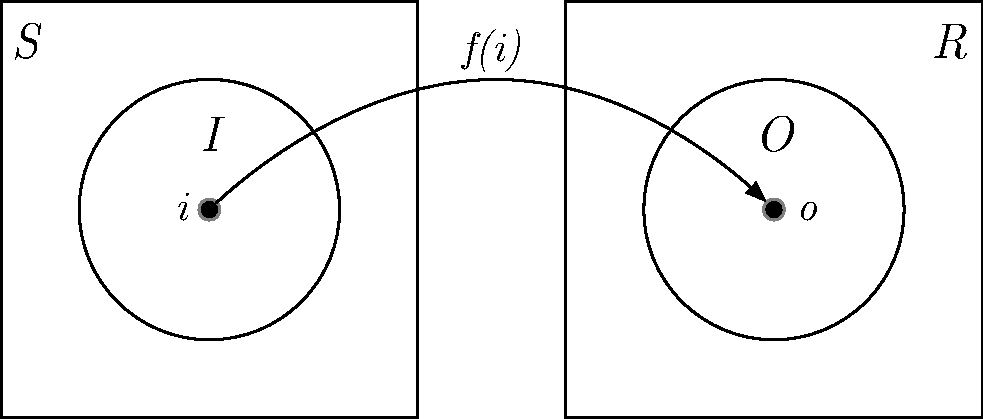
\includegraphics[width=22em]{stim_and_obs}
  \caption{Stimuli and observations: $S$ is anything that can change the observable behaviour of the SUT $f$; $R$ is anything that can be observed about the system's behaviour; $I$ includes $f$'s explicit inputs; $O$ is its explicit outputs; everything not in $S \cup R$ neither affects nor is affected by $f$.}%
  \label{fig:test_activity}
\end{wrapfigure}

The use of the terms ``stimulus'' and ``observations'' fits various test scenarios, functional and non-functional.
As depicted in \figurename~\ref{fig:test_activity}, a stimulus can be either an explicit \emph{input} from the tester, or an environmental factor that can affect the SUT\@.
Stimuli include, among others, the platform, the language version, the resources available, interaction with an interface, etc.
Observations encompass anything that can be discerned and measured like the content of a database, the visual responses on a computer screen, the time passed during the execution, etc.

Testing is about stimulation and observation, so we talk about \emph{test activity sequences} that are comprised of at least one stimulus and one observation.
But testing is also about verifying that the observed responses, the behaviour, match to ones that were previously defined.
This checking part is done by another actor:

\begin{definition}[Test Oracle]
  A test oracle $D : T_A \mapsto \mathbb{B}$ is a partial function from a test activity sequence to true or false.
\end{definition}

An oracle can be defined using different methods: a set of specifications an expected value for a variable after the execution of a particular test activity sequence, the expectation of an absence of crash, etc.

A test oracle is a partial function because it can leave certain elements of the SUT's behaviour unspecified.
This part of uncertainty is fundamental in the real world because systems have grown to be so complex that humans cannot anticipate all the reactions of the SUT in all environments.
It is useful nonetheless to have a name for a theoretical oracle that would have an answer for every possible question:

\begin{definition}[Ground Truth]
  The ground truth oracle, $G$, is a total test oracle that always gives an answer.
\end{definition}

This allows us to define two properties for all oracles:

\begin{definition}[Soundness]
  The test oracle $D$ is sound for test activity $a$ iff $D(a) \rightarrow G(a)$
\end{definition}
\begin{definition}[Completeness]
  The test oracle $D$ is complete for test activity $a$ iff $G(a) \rightarrow D(a)$
\end{definition}

A test oracle cannot, in general, be complete as it would require handling every possible test activity sequence.
It is not rare for an oracle to be unsound as humans can make errors writting specifications.

In practice, following pattern designs of modularity, the act of testing is composed of multiple test activity sequences that target specific elements of the SUT's behaviour:

\begin{definition}[Test Case]
  A test case $T_C$ is a test activities sequence that contains at least one stimulus and one observation with a test oracle that verifies each observation.
\end{definition}
\begin{definition}[Test Suite]
  A test suite is a collection of tests cases.
\end{definition}

In other words~\cite{bernot1991software}, a test case is a subset of inputs, and a subset of specifications from the ground truth that are matched against the trace of the test's execution.

Another concept that we will use when talking about software evolution is regression testing~\cite{yoo2012regression}:

\begin{definition}[Regression Testing]
  Regression testing is performed between two different versions of the SUT in order to provide confidence that newly introduced features do not interfere with the existing features.
\end{definition}

It is a way to avoid having a human write formal specification but the problem remains of trying every possible scenario and observing any useful response.

\todo{give some clues to each concept to tell why it is a field of research?}

% - - - - - - - - - - - - - - - - - - - - - - - - - - - - - - - - - - - - - - - -
\subsubsection{Levels of Testing}%
\label{sssec:levels_testing}
\begin{wrapfigure}{L}{25em}
  \centering
  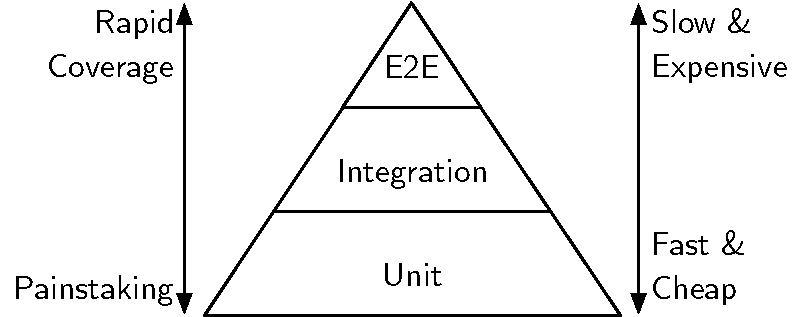
\includegraphics[width=25em]{test_pyramid}
  \caption{A view of the test pyramid.}%
  \label{fig:test_pyramid}
\end{wrapfigure}

In the case of software testing, the SUT can be different elements of a program, i.e.\ it can belong to different levels of abstraction.
One can decide to test a whole program, by manually giving inputs and verifying that the output is correct.
Or one could test individual functions, having a more control over the behaviour of each element.

These levels of test abstraction can be visualised with a test pyramid, as shown in \figurename~\ref{fig:test_pyramid}.
Tests are generally separated into three distinct categories.
The top category is for the End-to-End tests, which means testing the program as a whole.
It can mean interacting with the UI and evaluating the visual responses.
Whilst it allows for directly evaluating the well behaviour of the program, each test is costly in time and resources because the whole program has to be run.
Not only will each component be run, whether or not it requires testing, but time will also be spent on call to external libraries that are already tested.
At the other end of the test spectrum are the unit tests.
The goal is to test each and every component of the program (e.g.\ every function), as an individual and isolated from the rest of the program.
Running a single component is faster than running the whole program, but require much more work from the person writing tests, as every component needs its set of tests.
In between the two testing practices are the integration tests, which aim at ensuring the well collaboration of components \rephrase{work together as expected}, like verifying that gears rotate in the right way.
Examples of integration tests include API testing, or simply the fact of calling a function using the result from another function call.
This last example gives an intuition on how fuzzy the distinctions between all kinds of tests are, with definitions often relying on personal opinions\footnote{\url{https://testing.googleblog.com/2009/07/software-testing-categorization.html}}\footnote{\url{https://martinfowler.com/bliki/IntegrationTest.html}}.
More details about the loose definition of unit tests are given Section~\ref{sssec:unit_testing}.

The test hierarchy is often represented by a pyramid because it is generally advised to have many more unit tests than end-to-end tests.
Practitioners often recommend putting an emphasis on unit test, with a distribution of 70\% unit tests, 20\% integration tests, and 10\% end-to-end tests for example\footnote{\url{https://testing.googleblog.com/2015/04/just-say-no-to-more-end-to-end-tests.html}}.
More details on the strengths and weaknesses of unit tests are given in the next section, but we can convey some general truths here.
End-to-end tests require more maintenance as the software evolves, because test cases rely on many modules and their behaviour eventually change with time.
Also, with a broad coverage, it is difficult to identify components at fault in the case of a failing test.
Having unit tests for each component gives confidence that they behave accordingly and that if an integration test fails, the error lies in the interactions between the components.
Again, the broader the test, the greater the number of interactions which makes it difficult identifying the one at fault.
Because of this, the number of test levels has to increase alongside the software's growth --- e.g.\ grouping components into modules, modules into services, and services as the system.

Programs can be tested manually by a human (e.g.\ by interacting with the UI), but tests are generally automated to save time.
Automation often mean to programmatically describe a scenario, observations and their associated specifications.
Different levels can require different tools and frameworks\footnote{\url{https://martinfowler.com/articles/practical-test-pyramid.html}}.
For example, unit tests can be written in the same language as the main program, interacting with it like any other module (more details in the next section).
But to test a graphical user interface, one might need to run a window system and control the cursor's movements and clicks.

% - - - - - - - - - - - - - - - - - - - - - - - - - - - - - - - - - - - - - - - -
\subsubsection{Unit Testing}%
\label{sssec:unit_testing}

A unit test is supposed to target a precise component of the SUT, but defining the level of granularity is not trivial, even for experienced programmers\footnote{\url{https://martinfowler.com/bliki/TestPyramid.html}}\footnote{\url{https://martinfowler.com/bliki/UnitTest.html}}~\cite{runeson2006survey}.
In the case of a program written with an Object-Oriented language, such as Java --- we will put our focus on Java for the rest of this thesis --- the targeted component can be a class or just a method of a class.

\begin{listing}[H]
  \centering
  \begin{minted}[linenos,frame=topline,breaklines,highlightlines={3,5,7},highlightcolor=YellowOrange!20]{java}
public class TreeListTest {
    public void testIterationOrder() {
        TreeList tl = new TreeList(10);
        for (int i = 0; i < 10; i++) {
            tl.add(i);
        }
        ListIterator it = tl.listIterator();
  \end{minted}
  \begin{minted}[linenos,frame=bottomline,breaklines,firstnumber=last,highlightlines={11},highlightcolor=YellowGreen!20]{java}
        int i = 0;
        while (it.hasNext()) {
            Integer val = it.next();
            assertEquals(i++, val.intValue());
        }
    }
}
  \end{minted}
  \caption{Example of an object-oriented unit test (taken, and adapted for readability, from the Apache Commons Collections, in the class TreeListTest, line 270\protect\footnotemark): it consists of test inputs (lines 3--7) that manipulate the SUT\@; and assertions (line 11). Methods \texttt{.hasNext()} and \texttt{.next()} (lines 9 \& 10) are expected, implicitly, to behave correctly.}%
\label{lst:test_example}
\end{listing}
\footnotetext{\url{https://commons.apache.org/proper/commons-collections/xref-test/org/apache/commons/collections4/list/TreeListTest.html\#L271}}

An example of unit test is given in \listingname~\ref{lst:test_example}.
Tests are usually sorted in classes, and each test case corresponds to a method (which is why test cases are sometimes refered to as test methods, as we will encounter later on).
Specifications of expected values for observations are written using \emph{assertions}.
When the condition of an assertion is not met, we call it an assertion \emph{failure}, it raises an exception\rephrase{} and causes the test case to fail.
Assertions are a feature of test frameworks (i.e.\ internal DSL~\cite{fowler2010domain}), and allow test cases to be regular pieces of code.
This has advantages and disadvantages, it is easy to write test cases but might not be the most friendly\rephrase{} way to express a property on the software artifact targeted.
Test methods often rely on naming conventions to help the reader understand what is the target, and what behaviour it is checking.
Another pitfall to avoid is to test properties for the programming language used.

Unit tests are usually written by software engineers, as they are the one with the knowledge of the expected behaviour for the piece of software they have produced.
Large companies will also have test engineers, focusing on broader tests and commercially important features, as well as software engineers working on test infrastructure and tooling\footnote{\url{https://testing.googleblog.com/2016/03/from-qa-to-engineering-productivity.html}}.
Unit testing has becoming an integral part of modern software development with practices such as Test-driven Development (TDD)\footnote{\url{https://en.wikipedia.org/wiki/Test-driven_development}}~\cite{beck2003test} that consists in writing test cases first, and then writing code that complies.
Integrated development environments (IDEs) have been extended to make writing and reviewing tests easier.
Test automation in general is also a pillar of modern software delivery cycles like DevOps\footnote{\url{https://en.wikipedia.org/wiki/DevOps}}, with Continuous Integration (CI) tools that run test suites each time that code changes are pushed.
Tests can then be refined using exploratory testing\footnote{\url{https://testing.googleblog.com/2008/05/exploratory-testing-on-chat.html}}~\cite{kaner2000testing}, by trying to manually find flaws while documenting the process to then implement the results as test cases.
Manual testing is particularly useful to rapidly detect issues like slow response time, misleading error messages and other design concerns.

\begin{wrapfigure}[23]{R}{17em}
  \centering
  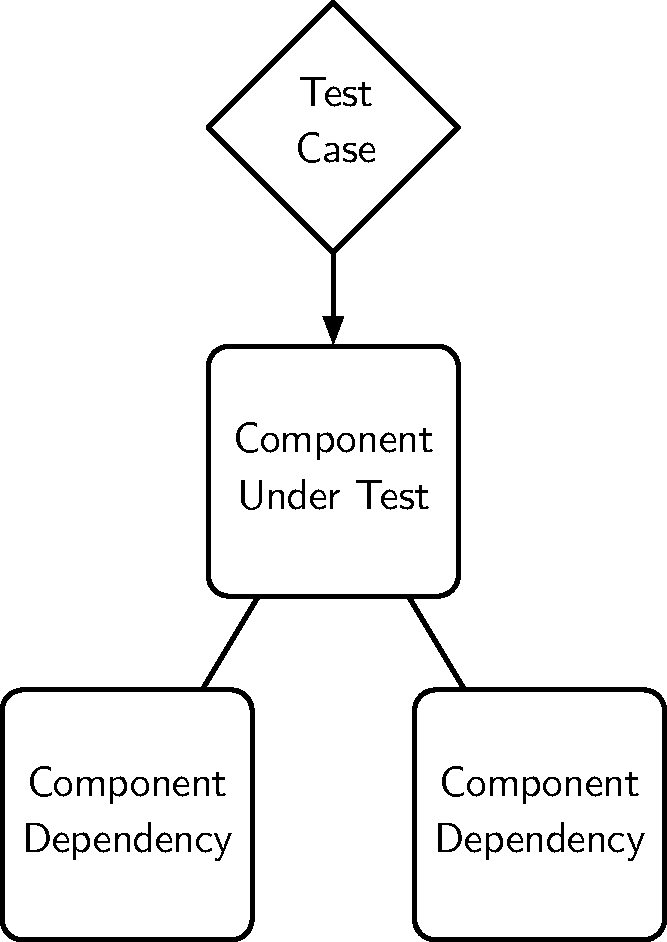
\includegraphics[width=17em]{component_dependency}
  \caption{Test target's dependencies.}%
  \label{fig:component_dependency}
\end{wrapfigure}

Because unit test are written with the same programming language as their target, certain features of the language --- that are supposed to help developers write clean code --- can become a hindrance.
A perfect example with Java are the private methods.
They exist because they enforce the separation of the public interface and the inner workings of a class.
But when one want to test a private method to make sure it does the right thing, it is not possible.
The alternative is to extensively test the public methods, making sure they trigger all sorts of behaviour in the private part of the class.
In this situation, we end testing a component that interacts with other components, as depicted in \figurename~\ref{fig:component_dependency}, but then it becomes a small integration test\footnote{\url{https://martinfowler.com/bliki/UnitTest.html}}.
The granularity of tests does not only depend on the needs and desires of the developer, but also on the limitations of the language.
Object-Oriented are particularly victim to this, as they are suited for composition design patterns~\cite{wolfgang1994design}, leaving no other option to the developer to try to limit interactions.
Ways to avoid writing test that trigger a long chain of reactions is to use doubles (or mocks) which are hand written clones of classes instances.\rephrase{}
Dependencies are also present in the test's code, as seen in \listingname~\ref{lst:test_example} with the lines 9 and 10, as other methods from the class under test can be used for the set-up or to retrieve certain observations.

Another common problem with testing are flaky tests.
A flaky test is a test which result is not deterministic.
There can be various causes for a flaky test, e.g.\ a direct usage of RNG function, or a crash happening only in scenario with a certain scheduling in the case of parallel applications.
The advantage of small tests with controlled interaction with the environment is that they are less likely to be flaky.
This a hard problem\footnote{\url{https://testing.googleblog.com/2017/04/where-do-our-flaky-tests-come-from.html}} as flaky tests can be (i) hard to identify, (ii) hard to refactor, and (iii) hard to avoid in the first place.

\todo{how do you know you have a good oracle}

\begin{listing}
  \centering
  \begin{minted}[linenos,frame=lines,breaklines]{java}
import org.junit.Test;
import static org.junit.Assert.assertEquals;

public class MyTests {
    @Test
    public void multiplicationOfZeroIntegersShouldReturnZero() {
        MyClass tester = new MyClass();
        assertEquals(0, tester.multiply(10, 0), "10 x 0 must be 0");
    }
}
  \end{minted}
  \caption{Example of a JUnit test class. A test class is simply a group of test methods (i.e.\ test cases). Each test case is identified by the annotation \mintinline{java}{@Test}.}%
\label{lst:junit_example}
\end{listing}
An example of test framework, for Java, is JUnit~\footnote{\url{https://junit.org/}}.
The basic structure of a JUnit test class is given in \listingname~\ref{lst:junit_example}.

\todo{\footnote{\url{http://blog.codepipes.com/testing/software-testing-antipatterns.html}}}

% --------------------------------------------------------------------------------
\subsection{Elementary Metrics}%
\label{ssec:elementary_metrics}
Metrics have been developed to help developers automatically assess the quality of their code.
Each metric measures one specific characteristic, such as the need for refactoring, the size of the program, or --- and we are particularly interested in this one --- the likelihood of bugs.

\begin{figure}
  \centering
  \fbox{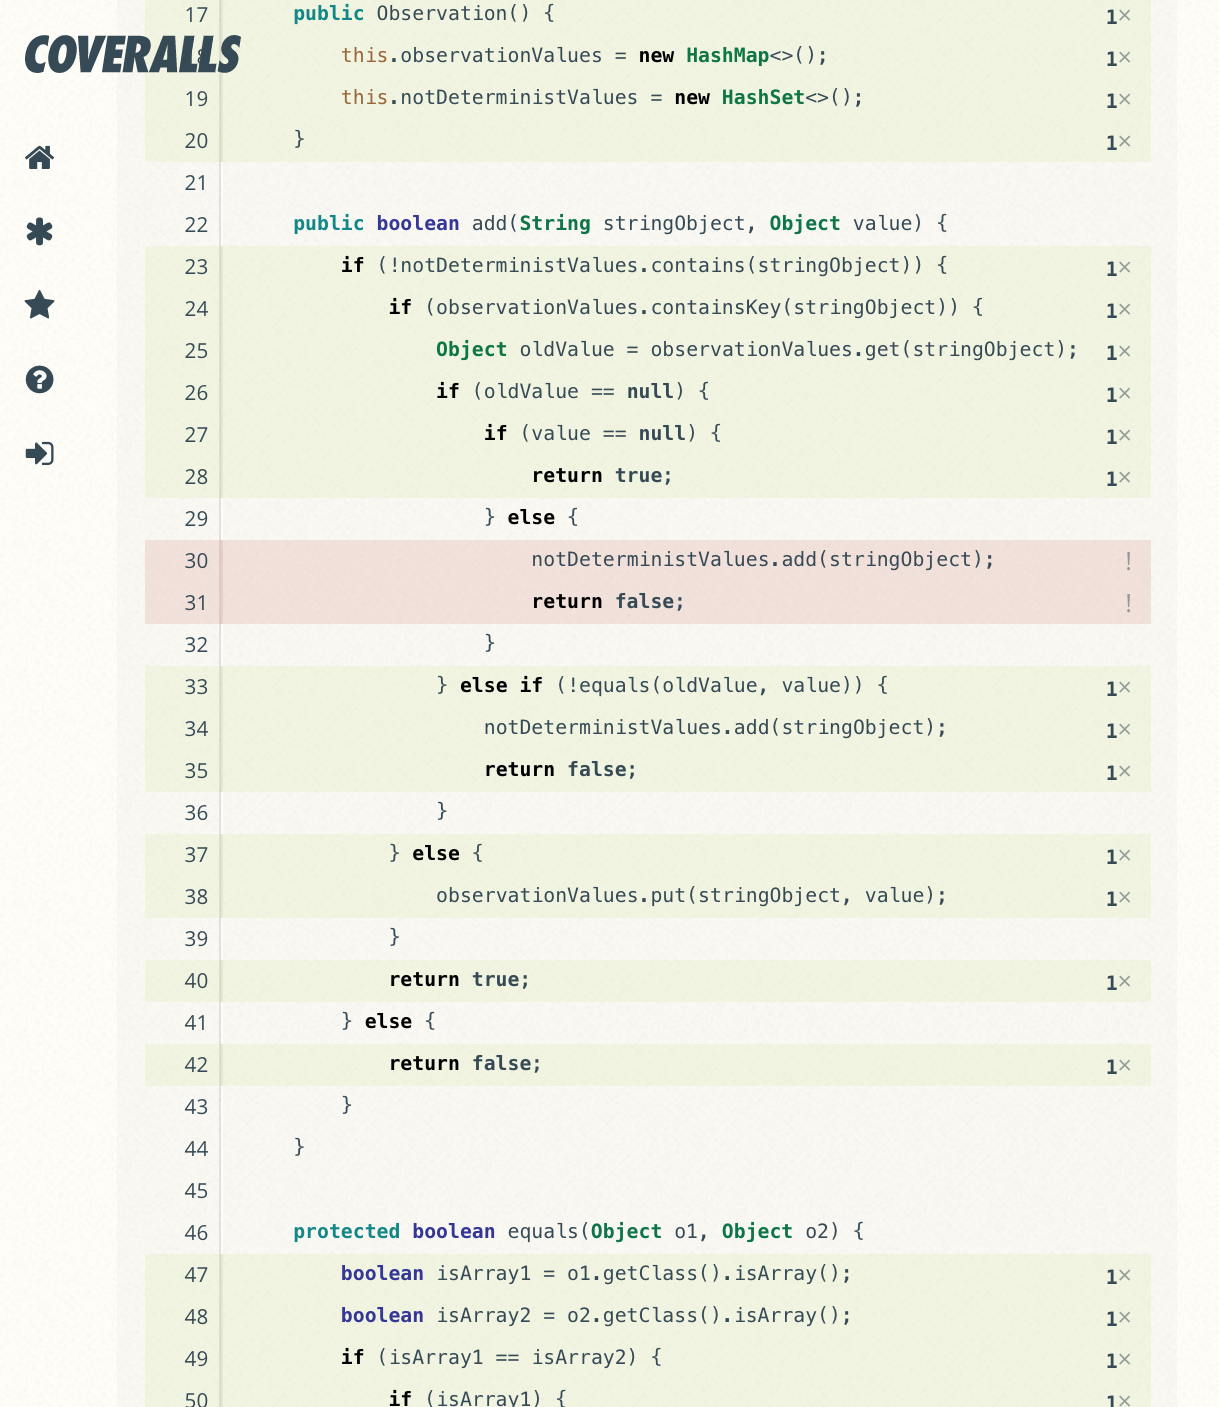
\includegraphics[scale=0.80, trim=5.1cm 10.2cm 1.5cm 3.7cm, clip]{screenshot_coverage}}
  \cprotect\caption{Example of coverage reporting from the Coveralls\protect\footnotemark{} tool. We can see that the statements in the first \texttt{else} branch have not been executed a single time. The numbers on the right represent the number of times each line has been executed.}%
  \label{fig:screenshot_coverage}
\end{figure}
\footnotetext{\url{https://coveralls.io/}}

The most basic metrics to measure how thoroughly tested a system is, are coverage based metrics.
For example, during the test suite execution, one can keep track of all statements that were executed.
At the end, you have a percentage of executed statements for the total number of statements.
Instead of statements, one can also keep track of control flow branches explored.
\todo{give examples for other metrics?}
These metrics, especially the statement coverage, are wide spread in the industry --- with coverage tools integrated out-of-the-box with source code hosting services and continuous integration services.
An example of coverage visual report is shown in \figurename~\ref{fig:screenshot_coverage}.

It is generally acknowledged that a system with high coverage means that the system is less likely to have bugs --- but it is not foolproof~\cite{hovemeyer2004finding,inozemtseva2014coverage}.
Such simple metrics are not good at pointing out corner cases\footnote{\url{https://martinfowler.com/bliki/TestCoverage.html}}.
If we take the following example \texttt{if ($C_1$ AND ($C_2$ OR $C_3$))} and $C_3$ makes the program crash, then it is possible to explore both branches without executing $C_3$.
\todo{What are their limits}

A drawback of metrics is that in practice, testers will change behaviour once they know how the measurement works\footnote{\url{https://testing.googleblog.com/2009/09/7th-plague-and-beyond.html}}.
They will write tests that will perform well for a given metric and ignoring other important factors (e.g.\ diversity\footnote{\url{https://testing.googleblog.com/2009/06/by-james.html}}~\cite{baudry2014diversify,baudry2015multiple}).
In these cases the metric has become the goal instead of a progress measurement.

% --------------------------------------------------------------------------------
\subsection{Mutation Testing}%
\label{ssec:mutation_testing}
\begin{wrapfigure}[23]{L}{9em}
  \centering
  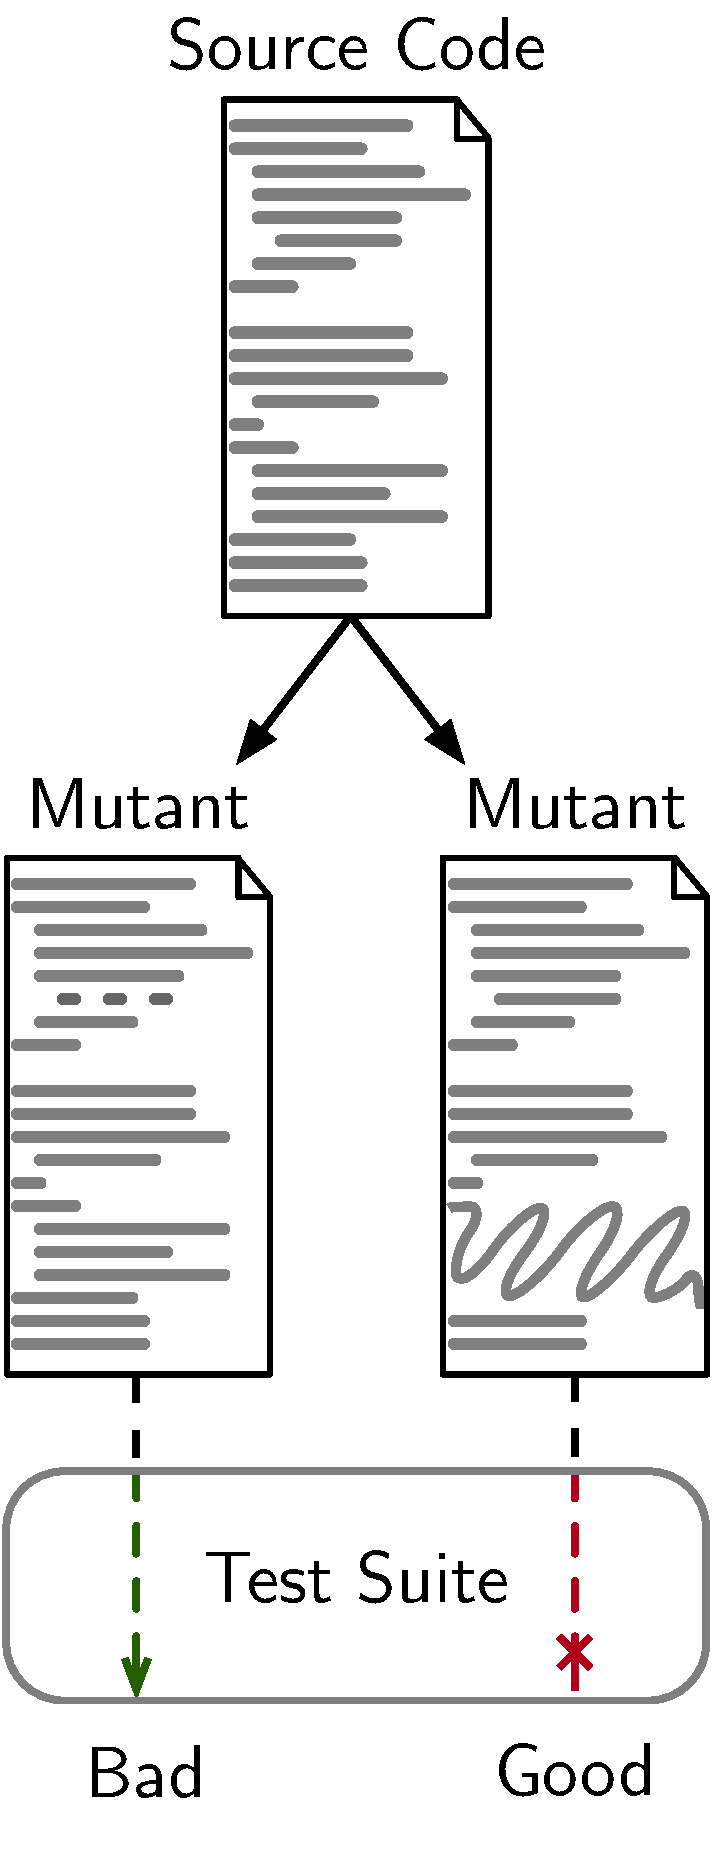
\includegraphics[width=9em]{mutation_testing_report}
  \caption{Mutation testing process.}%
\label{fig:mutation_testing}
\end{wrapfigure}
% Introduction
Mutation testing is a method used to assess the quality of a test suite, giving it a grade called \textit{mutation score}.
The idea is to insert bugs in the software and see if these faulty versions still pass the tests or not.
We call the derived versions \textit{mutants}, hence the name mutation testing.
When a mutant goes through the test suite without making a single test fail, it is considered \emph{live}, and the opposite case it is considered \emph{dead}.
The global process is depicted in~\figurename~\ref{fig:spaces}.
The main appeal is that, a test suite with a good mutation score, in addition to ensure the well behaviour of the SUT in useful scenarios, it can detect bad behaviours --- which is particularly useful for regression testing.\rephrase{}
There is a correlation between mutation score and coverage score as test suites with high mutation score tend to have good coverage~\cite{assylbekov2013investigating}.
In general, mutation coverage can be seen as a line coverage with levels of coverage depending on the number of mutants present in this line, similarly to the number of times the line is executed.
It has been found that correlations between mutation scores and real fault detection are weak~\cite{papadakis2018mutation,just2014mutants}.
Mutation testing has been extended in various directions (e.g.\ specification mutation) but we are focusing on the primary usage, the evaluation of a test suite for a given implementation.

\addref{fundational papers}

% \todo{applying the mutation on the source code instead of modifying the runtime makes it easier to detect~\cite{danglot2017correctness}}

% Mutators
Mutants are obtained by applying \emph{mutators} on the original version.
These operators can be varied, from fine-grained like changing a condition (e.g.\ substituting $\leq$ with $>$), to the granularity of classes~\cite{segura2011mutation} (e.g.\ delete the body of a method \addref{descartes}).
Running first mutation testing with large operators allows to rapidly detect gaps in the coverage of the test suite for unit testing but also for integration testing.
Fine grained mutation can then be employed to meticulously evaluate the functional testing capabilities of the test suite~\cite{howden1982weak}.
Most of the time, we generate 1-\emph{order} mutants, that means that a mutant is the result of a mutator applied once.
A mutator will usually generate several mutants.
For example, a mutator that replaces a \texttt{while} statement into a \texttt{do-while} statement will generate a mutant for each \texttt{while} in the artifact.
In the case of $k$-order mutants, which can be thought of as the result of $k$ succesive 1-order mutants\cite{wah2000theoretical}, the number of derived programs starts to blow up.

% Difficulties
Mutation testing suffers from drawbacks that have limited its use outside of the research world even though it has been an active research domain for many years~\cite{jia2011analysis}.
The first obvious flaw is that it is slow.
For compiled languages, all mutants have to be compiled, and that process often takes a lot of time for large programs.
Then the whole test suite has to be executed for each mutant, which again is a long process.
However, given certain trade-offs in terms of quality of the mutation analysis process (e.g.\ not generating all possible mutants), the computational complexity can be dodged~\cite{offutt1993experimental,movzucha2016mutation}.
Optimized techniques for regression testing also exist~\cite{yoo2012regression}, including minimisation, selection and prioritisation, which can reduce the execution time of the test suite.
The mutant generation is also full of traps.
The major pitfall that cannot be avoided is the equivalent mutant problem.
Some mutants, although they have a different program than the original, have the same semantics.
Which means that they will always pass the test suite and will not bring any insight on the SUT\@.
The generation of mutants that are simply syntactically valid is also a non-trivial problem that requires pattern replacement instead of simple text replacement~\cite{simao2009transformational}.

Another difficulty for mutation testing to take on in the industry is the lack of understanding by practitioners.\rephrase{}
The process of mutation and elimination can be confusing.
But also, when a mutant is live, it is not always clear what actions should be taken in order to kill it.
\todo{maybe add more}

% Pitest
Multiple mutation tools exist, with differences on the level of abstraction they handle, different performances and different correlation with real fault detection.
Many of them are robust thanks to the efforts from the research community to reach the industry and the need to have reliable implementations to do\rephrase{} empirical studies related to mutation testing.
One of these tools is PIT\footnote{\url{http://pitest.org/}}~\cite{coles2016pit}, a tool for the Java bytecode.
The research version (i.e.\ state-of-the-art) of PIT is known to perform better than its competitors overall~\cite{kintis2017effective}.
Two technical details are interesting for us.
The first one is the way it stores the mutants generated.
The location of a mutant is specified by (i) the name of the method and class, (ii) the method signature and (iii) the instruction on which the mutation occurs.
This little information is sufficient to recreate each mutant while having a small storage footprint.
The other important detail is that PIT is deterministic.
That is, for the same program, the same mutants will always be generated, and thus the mutation score will always be the same.

\begin{wrapfigure}[15]{R}{23em}
  \centering
  \fbox{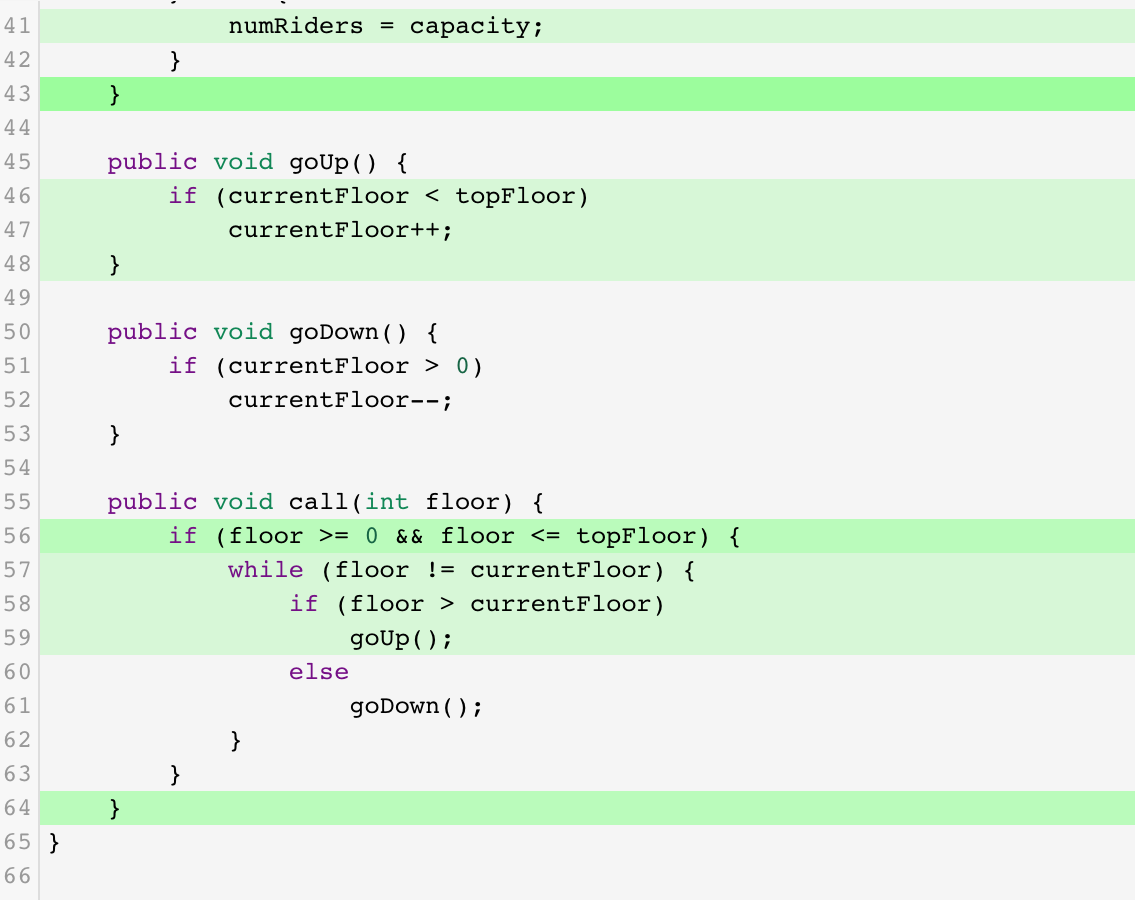
\includegraphics[scale=0.75,trim=1.8cm 1.4cm 6.9cm 8.6cm, clip]{screenshot_mutation_coverage}}
  \caption{Example of mutation coverage reporting from Code Defenders\protect\footnotemark{}~\cite{rojas2017code}. Shades of green are used to denote the amount of testing for a line.}%
  \label{fig:screenshot_mutation_coverage}
\end{wrapfigure}
\footnotetext{\url{http://code-defenders.org/}}
The way mutation testing tool report their result is interesting.
Instead of trying to show each statement that has been mutated, and inspired by reports of line coverage, they usually display a regular line coverage report with shades of colour.
The lightest means that the line has been executed, and the darker it gets, the higher the number of mutants located in this line.
An example of mutation coverage visual report is shown in \figurename~\ref{fig:screenshot_mutation_coverage}.

% --------------------------------------------------------------------------------
\subsection{The Need for Easy-to-use Tools}%
\label{ssec:need_easy}
Software Engineering, as a research field, being tightly coupled with practices in the industry, it is important to understand the attempts at transfering research knowledge to the industry.
There are many reasons to help the industry, for example: reducing the risks of bugs in critical systems, automating the development process, etc.
One way researcher often go, is to develop a tool and then try to introduce it in the workflow of practictioners.
But even with good intentions, the process of acceptance by practitioners for a research product is often complicated~\cite{delahaye2015selecting}.

An issue that is often faced, is the difficulty for practitioners to understand the usage of the tool, or even its purpose.
Thus, not only should a researcher consider the amount of bugs their tool can detect, they should also make sure it is accessible and easy to understand.
Having an easy-to-use tool can also open new paths for research, reveiling new problems, and making studies with professional developers easy.

Valuable experience has been earned from static analysis researchers' attempts at integrating their tools in the workflow of their engineer colleagues~\cite{bessey2010few,sadowski2015tricorder,sadowski2018lessons}.
Each false positive undermines the trust developers have in the tool.
Each misunderstood error make developers angry.
And each warning that do not \emph{feel} relevant to the developer raise the likelihood that future warnings will be ignored.
As humans, we avoid change unless it is necessary or is directly beneficial to us.
Developers do not want to be slowed down by additional actors in their workflow, and companies do not want additional cost with little return.

The field of software testing, in which this thesis is set, is no stranger to this problem.
Tests are, in most cases, written and maintained by general software engineers.
Thus, we must aim at producing tools with little overhead and fully integrated with popular test frameworks --- making it easy for developers to try the tool to see if it fits their needs, and, if they incorporate it in their workflow, it brings important data to demonstrate the scientific value of the tool.

% --------------------------------------------------------------------------------
\subsection{Cognitive Support Tool Development}%
\label{ssec:cognitive_support}
\todo{}

Acceptance of a tool, outside of the research world, depends on many parameters, including its accessibility.
In this section we describe how a tool can be designed to fit this requirement.

Research has been done on designing tool that do not overwhelm users (e.g.\ designing interfaces~\cite{oviatt2006human}) and theories on design processes have been developped.
The grounded theory~\cite{stol2016grounded}, for example, argues for an iterative design process, by refining the product based on data and feedback from users.

Tools, including SBST, need a high level on interactivity with the developers, to guide the search process (to inject domain knowledge, to select useful objectives, etc.)~\cite{marculescu2017transferring}

Another method of evaluation that should not be dismissed are case studies~\cite{flyvbjerg2006five}.
\todo{}


% ================================================================================
\section{Test Suite Amplification}%
\label{sec:test_suite_amplification}
In this Section, we provide more context for this thesis' contribution.
We explain how global optimization techniques, including metaheuristic search techniques (e.g.\ genetic algorithms) can be applied to software engineering problems --- for example, by using software metrics as target functions.
Section~\ref{ssec:genetic_improvement} presents how source code can be manipulated for search processes, and Section~\ref{ssec:test_amplification} presents the specific problem of improving test suites.
Section~\ref{ssec:dspot} introduces~\dspot{}, a tool that enhances tests for a better coverage, and for which this thesis can be seen as an extension.\rephrase{}

% --------------------------------------------------------------------------------
\subsection{Genetic Improvement}%
\label{ssec:genetic_improvement}
\todo{}

Genetic improvement (GI)~\cite{petke2017genetic} uses automated search to find improved versions of existing software.
Automated search encompasses optimisation methods that approximate optimums (e.g.\ genetic algorithms, simulated annealing).
Applying search-based techniques for software engineering problems is not new~\cite{mcminn2011search} as is the field of genetic programming (GP)~\cite{koza1994genetic} (with, at the time of writing this thesis, comprises over 12000 references\footnote{\url{http://www.cs.bham.ac.uk/~wbl/biblio/}}).
But from around 2012, when the name of GI has been coined~\cite{harman2012gismoe}, the reached level of computing power that one can easily have access to has allowed research to achieve impressive results (e.g.\ transplanting a feature from one program to another~\cite{barr2015automated}).

\addref{fundational papers}

Evolutionary methods are known to come up with creative solution for problems with complex search space~\cite{lehman2018surprising}, and programming tasks often require creativity and knowledge that only human can master.

Search operators are most frequently \emph{delete}, \emph{copy} and \emph{replace}~\cite{petke2017new}.
For example, duplicate a line of code, or delete a method call, or replace an integer by another number.

One thing to remember, is that complex search techniques are not always the most efficient~\cite{shamshiri2017random}, as a simple random search can sometimes produce sufficient results.
This is especially true for object-oriented test generator, as they consist of sequences of object constructor and method calls, and it can be hard to know how to combine them to pursue a certain coverage goal.
Synergy between method calls is hard to predict because classes are interlinked, methods have side effects, and there are goals that cannot be reached.
In addition, having a specific goal in mind can be at the expense of a wider coverage.

% --------------------------------------------------------------------------------
\subsection{Test Amplification}%
\label{ssec:test_amplification}
As unit tests are program artefacts like others, GI can be applied on test suites~\cite{danglot2017emerging}\addref{A Systematic Literature Review on Test Amplification} and search techniques have been employed since 2005~\cite{baudry2005automatic}.
It is relatively recent compared to works tackling the problem of Test Data Generation (i.e.\ generating tests from scratch for a piece of software), but it is only recent that we can expect software projects, large or modest, to come with strong test suites.
Various goals can be pursued to improve a test suite, from automated refactoring to improve a specific metric, to enhancement of existing tests to fill the often partial coverage\footnote{\url{https://testing.googleblog.com/2014/07/measuring-coverage-at-google.html}}.
The term of test \emph{amplification} is used to denote the process of processing and extending tests to reach further targets.
Baudry et al.~\cite{baudry2005automatic} wrote a tool for \CS{}\rephrase{} to explore more of the input space and improve the mutation score.
Yoo et al.~\cite{yoo2012test} proposed the Test Data Regeneration (TDR) method for creating equivalent tests with different inputs --- particularly useful for fault detection and avoiding overfitting (when the SUT passes the tests but does not behave correctly in the general case).
Xuan et al.~\cite{xuan2015dynamic,xuan2016b} created a tool to refactor test suite to improve dynamic analysis and fault detection.

% --------------------------------------------------------------------------------
\subsection{\dspot{}}%
\label{ssec:dspot}

\begin{figure}
  \centering
  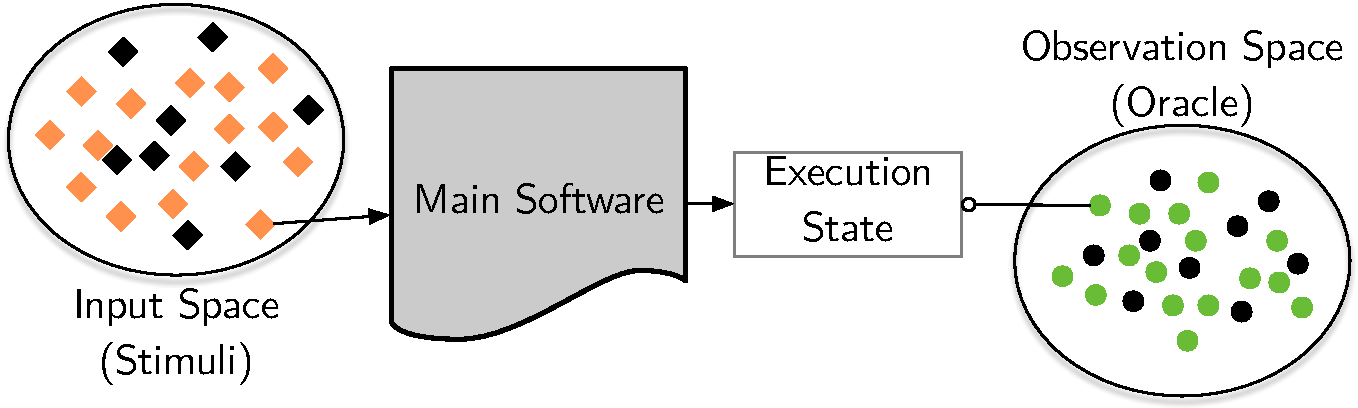
\includegraphics[width=36em]{spaces_report}
  \caption{On the left, the testing input space is composed by specified input points (orange diamonds) and unspecified input points (black diamonds). On the right, the observation space over a given program state depicts the assertions of tests. The green circles are values that are already asserted in the existing test suite, the newly added assertions are shown as black circles.}%
\label{fig:spaces}
\end{figure}

\dspot{}\footnote{\url{https://github.com/STAMP-project/dspot}}\addref{Genetic-Improvement based Unit Test Amplification for Java}\cite{baudry2015automatic,baudry2014tailored,baudry2015dspot} is a test amplification tool.
Its goal is to amplify tests individually to improve a given metric, e.g.\ mutation score.
Going back to our definition of tests, with the notions of stimuli and observations, \dspot{} has a search process on both spaces.
New inputs are generated, and new observations are made.
A visual representation is given in \figurename~\ref{fig:spaces}.
Because of the oracle problem, \dspot{} focuses on regression testing --- assertions (i.e.\ specifications) are generated from observations of an actual execution of the test.
It is a Java tool, it uses Spoon~\cite{pawlak2016spoon} to manipulate the source code, and consists in about 14000 physical lines of code (i.e.\ non-comment and non-blank).

To explore more of the input space (we also talk about \emph{amplifying} inputs), operators called I-Amplification are applied.
\begin{description}
  \item[\textit{Amplification of literals}] Similarly to TDR, literals (numeric, boolean, string) are replaced by neighbours. For example, an integer can be multiplied by 2 or a random character can be added to a string.
  \item[\textit{Amplification of method calls}] Methods calls can be duplicated, removed, or made-up by picking a random variable in the test and calling one of its methods with random parameters.
  \item[\textit{Test objects}] If a new object is required for an amplified method call, one of the appropriate type will be built by using the default constructor.
\end{description}
Like 1-order mutants, only one amplification is applied at a time, to limit the number of generated tests.
Because the random amplification can create flaky tests, they are executed three times to verify that they have a consistent behaviour.

As for the amplification of observations (A-Amplification), focus is put on checking more properties to kill more mutants.
Assertions are generated as follows: the state of program is collected after execution of the test case to know the actual values and use these values as oracle.

The global amplification process is as follow:
\begin{enumerate}
  \item remove all assertions, but keeping the method calls used for the assertions' arguments to make sure the test triggers the same behaviour;
  \item execute the test with instrumentation to collect the values from getter methods, and then generate assertions with the values from the observations;
  \item generate multiple tests by applying input amplifiers;
  \item create new assertions if possible;
  \item compute the mutation score, noting the tests that have a higher score;
  \item if the amplified test raises an exception, a \texttt{try/catch} statement is added around the whole test to catch this exception, and at the end of the \texttt{try} block, a \texttt{fail} statement is added to make sure the exception is raised all the time; and
  \item repeat a certain amount of time.
\end{enumerate}

Using mutation score as the target metric allows us to see the problem of amplification as a problem of finding bugs.
In other words~\cite{shamshiri2015automatically}, the amplification process consists of improving the code coverage to execute faulty statements, and improving the propagation of faulty program states to an observable output.

\dspot{} is different from traditional test generator like EvoSuite~\cite{fraser2011evosuite} for multiple reasons.
It is more than just using the existing test suite as a good starting population.
\todo{}
\cite{rojas2017detailed}

The result of \dspot{} is a set of amplified tests but it should not stop there.
Building incrementally on top of humans work is valuable.
Adding the generated tests in the main test suite has multiple advantages.
First, is the review process.
Developers have to review changes before it is accepted in the main code.
During the review process developers can tweak the assertions, rearrange the inputs, etc.
In that sense, \dspot{} fits as a software development bot, integrated in the workflow~\cite{urli2018design}, that could be run on code changes, after making sure the test suite is passing.
The amplified tests would then be submitted as a Pull Request (a.k.a.\ Merge Request) in the code version control platform used.
Secondly, it is more efficient.\todo{}


% ================================================================================
\section{Problem Statement}%
\label{sec:problem_statement}
This thesis aim at helping developers understand amplified unit tests.
There are two sides for this problem: supporting the developer understand the test (Section~\ref{ssec:need_doc}) and cleaning the tests from the noise injected during the amplification process (Section~\ref{ssec:random_noise}).

% --------------------------------------------------------------------------------
\subsection{The Need for Unit Test Cases Documentation}%
\label{ssec:need_doc}
The first challenge in rendering generated tests comprehensible, is to bundle them with explanations, like we do by documenting the code we write.
Several works have already highlighted the need for test documentation, with developers surveys~\cite{daka2014survey,prado2015wap,prado2016advances,prado2018towards,li2016automatically} and experiments~\cite{panichella2016impact} to measure the added value of documentation.
Even when they are short, tests can be complex and hard to understand.
In all cases, having documentation --- which include documentation comments like JavaDoc, but also the naming of the tests and variable --- has many advantages\footnote{\url{https://testing.googleblog.com/2014/10/testing-on-toilet-writing-descriptive.html}}~\cite{daka2017generating}, especially for generated tests~\cite{rojas2017search,shamshiri2018how}:
\begin{itemize}
  \item faster to get familiar with the test;
  \item faster fault localisation (e.g.\ figuring out if there is a bug in the test or the SUT) when the test fails; and
  \item helps to build trust in a test generator if it can provide a proof for its result.
\end{itemize}

Information to understand can be divided into four categories: (i) the component targeted; (ii) the context of the test method; (iii) the actual piece of code (i.e.\ the logic) that is the test method; and (iv) the properties checked.
And we can split them again in two groups: the \emph{what} and \emph{why} informations.
As we will see in Section~\ref{sec:related_works}, extensive works have been produced to generate automatic documention of the what information.
As for the why information, it is difficult to automatically extract the motivation of the developper that wrote the test.
But in the case of generated test, we have the reason why they were kept: they bring something to the metric.
Thus, if we focus on amplification for mutation score, we would need to explain this score and what new mutants are killed.
A lack of works on assisting humans to get the grasp of a mutation score makes a good case for us to tackle the problem of explain a killed mutant.

In source code management platforms, pull requests (through which amplified are submitted for review and merge in the main branch) are accompanied by textual descriptions.
Given that amplified tests should, in most cases, extend an existing test --- that we can suppose have documentation already --- the explanation of the added value of the amplification would fit in the pull request description.
It is important to restrict the scope to simple text, as it would not require a change in developers workflow.

% --------------------------------------------------------------------------------
\subsection{The Generated Random Noise}%
\label{ssec:random_noise}
Through the search process, noise is injected in the test case.
This problem of ugly generated tests code is a shared problem between all kinds of generators~\cite{rojas2017search}.
Generated tests are equally helpful than hand-written tests (with randomized names) for software maintenance tasks~\cite{shamshiri2018how}\todo{\cite{grano2018empirical}}, but don't seem to find more bugs~\cite{fraser2015does}, based on the limited data available.
So the goal is to make a similar job than humans, and because documentation is not sufficient to understand and review the code, tests need to be clean and logical to speedup the comprehension process.
Even though it has been known for a long time that the amount of time needed by developers to locate and understand code is frequently greater than the amount of time that they spend making modifications~\cite{ko2006exploratory}, existing works have largely focused on best efforts.

On a side note, in many modest projects, unit test are used as examples of the program's usage, and sometimes they replace traditional documentation.
In those cases, developers put a lot of efforts in making tests easy to understand.
Doing part of that chore automatically would remove part of the burden for humans.


% ================================================================================
\section{Related Works}%
\label{sec:related_works}
In this section we review the large body of related works from the domain of software maintenance~\cite{swanson1976dimensions}.
We are interested in tools that automatically generate documentation --- and there are many of them, as it is well-known that software documentation is important~\cite{de2005study} (even for modern agile methods) but it is time-consuming, often times poor and incomplete~\cite{briand2003software}, and is hard to maintain~\cite{forward2002relevance}.
They range from documenting general purpose source code (Section~\ref{ssec:doc_generation}), to commit message generation (Section~\ref{ssec:commit_generation}), and documenting test cases (Section~\ref{ssec:test_doc}).

% --------------------------------------------------------------------------------
\subsection{Source Code Documentation}%
\label{ssec:doc_generation}
\todo{these works are useless, why describe them?}

Works on source code documentation --- also called software artifact summarisation --- often consist of retrieving information from the source code to then arrange this information in a way that is easier and quicker to grasp for a human.
This section does not aim at providing a survey of the field (for which there are already, including automatic summarisation~\cite{jones2007automatic,nazar2016summarizing}, natural language paraphrasing~\cite{neubig2016survey} and automatic comment generation~\cite{wang2018comment}), but to present the general techniques used as well as the kind of results those tools produce.

As said above, such tools will rearrange information, stripping irrelevant pieces, summarising chucks on code, and put central information on the front.
In other words, they render the what information in a human comprehensible way --- they \emph{paraphrase} the code.
This is the main reason why, even automatic summarisation of natural language documents has been attempted by researchers for more than half a century~\cite{jones2007automatic}, finding a link with our problem of explaining the why information is not trivial.

\begin{table}
  \centering
  \begin{tabular}{llll}
    \toprule
    \multicolumn{2}{c}{Structural} & \multicolumn{1}{c}{Collaborational} & \multicolumn{1}{c}{Creational} \\
    \multicolumn{1}{c}{Accessor} & \multicolumn{1}{c}{Mutator} & & \\
    \midrule
    Get & Set & Collaborator-Accessor & Constructor \\
    Predicate & Command & Collaborator-Mutator & Copy-Constructor \\
    Property & & & Destructor \\
     & & & Factory \\
    \bottomrule
  \end{tabular}
  \caption{A taxonomy of method stereotypes.}%
  \label{tab:dragan_taxonomy}
\end{table}

One of the most influential works was produced by Dragan et al.~\cite{dragan2006reverse,dragan2011emergent}, which is about method stereotypes.
They proposed a taxonomy of \CC{} methods, given in \tablename~\ref{tab:dragan_taxonomy}, and a way to automatically assign stereotypes.
This way of annotating methods lead to other works --- using stereotype distribution as a signature descriptor for systems~\cite{dragan2009using}, extending the taxonomy for Java methods and classes~\cite{moreno2012jstereocode}.

Buse and Weimer~\cite{buse2008automatic} wrote a tool to automatically document the exceptions a method can raise.
Exceptions are dugged up from the call stack and the conditions for them to be raised are translated in natural language.
They compared their generated documentation with hand-written documention in a survey with developers.

Hill~\cite{hill2009automatically,hill2010integrating} has developed a model, the Software Word Usage Model (SWUM), that captures the occurrences of words in code, and also their linguistic and structural relationships.
\say{SWUM captures the conceptual knowledge of a programmer expressed through both natural language information and programming language structure and semantics, in the form of phrasal concepts. In contrast to existing lexical approaches, we take a transformative step in automatic analysis for software engineering tools by accounting for how words occur together in code, rather than just counting their frequencies.}
Because programmers tend to choose descriptive and meaning names for code units~\cite{liblit2006cognitive}, natural language descriptions of code artefacts can be made, without necessarily having to understand the code.

Sridhara et al.~\cite{sridhara2010towards,sridhara2012automatic} worked on automatically generating summary comments for Java methods.
For that they wrote an algorithm to extract important code statements and used SWUM to paraphrase those statements.
They did a survey with developers to evaluate the accuracy and usefulness of their contribution.

McBurney and McMillan~\cite{mcburney2016automatic} wrote a tool to generate natural language descriptions of the context of Java methods.
What they call context is how the methods are invoked.
They use the SWUM to describe the method, describe the method's caller, what the return value is used for, what methods it calls, and how the return value can be used.
They did two user studies.

Sridhara et al.~\cite{sridhara2011automatically} worked on describing methods from a high level point of view.
They detect high level actions (i.e.\ statements grouped by a loop or a condition) and use the SWUM to describe them.
They did a survey with developers to judge the descriptions synthesised.

Moreno et al.~\cite{moreno2013automatic} developed a tool to automatically generate summaries of Java classes.
A summary is composed of the class' stereotype~\cite{moreno2012jstereocode}, a description of its interface, structure and behaviour (by enumerating the most important methods).
Summaries are in natural language and generated using templates.
They did a survey with developers to judge how readable and understandable the summaries are.

Rastkar et al.~\cite{rastkar2010summarizing} worked on summarising bug reports, including involved discussions.
They label sentences and extract individual information.
Works related to bug reports are important for us as a killed mutant is a bug in a certain way --- but the knowledge we can extract from these works is not obvious because part of the job of a bug report is to help localise the bug, and in the case of mutation testing we already know the source.
Nevertheless, we can learn from these works how to explain the repercussions of a mutant.
Except that in this case, it is focused on summarising a discussion.\rephrase{}

% --------------------------------------------------------------------------------
\subsection{Source Code Change Documentation}%
\label{ssec:commit_generation}
Software evolves, iteratively, line by line, commit by commit.\rephrase{}
Past the phase of assimilation when a developer first start to work on a project, a significant part of the job consists of managing the growth of the project, making small changes to the code base without unwanted side effects, and reviewing commits.
Commits bundle a cohesive set of changes with a textual description, in which it is customary to provide some context, the motivation and possibly a digest of the changes --- part what and part why information.
Although developers view accurate and concise descriptions as useful, few put the efforts in writing such comments.
In consequence, researchers have written tools to automatically generate commit messages.

Dragan et al.~\cite{dragan2011using} proposed commit stereotypes.
Those stereotypes are composed of the modified classes and methods' stereotypes.
For example, a commit where 75\% of the added/deleted methods are factory methods denotes an ``object creation modifier''.

Cort\'es-Coy et al.~\cite{cortes2014automatically,linares2015changescribe} developed \textit{ChangeScribe}, a commit message generator.
From Git\footnote{\url{https://git-scm.com/}} changes they identify the responsibilities of the modified classes and methods, attribute stereotypes to changes~\cite{dragan2011using}, keep the most impactful (i.e.\ the most called modified methods or classes) changes, and generate natural language descriptions.
Messages are generated using templates.
The evaluated their tool with survey, comparing real-life commit messages and generated messages, asking the developers which one they prefered.
They also provide a table listing many approaches for generating descriptions of source code changes and software artifacts, providing more references than this section.

Jiang and McMillan~\cite{jiang2017towards} worked on generating one-phrase summaries of commits.
They used a classifier trained on real commits to label a commit with a verb (e.g.\ add, fix), identify the most important words occurring in the \texttt{diff}, and then use common phrase structure to combine the verb and the subject.

Jiang et al.~\cite{jiang2017automatically} used neural machine translation to generate a commit message from a \texttt{diff}.
Neural networks were also used by Loyola et al.~\cite{loyola2017neural}.

\begin{table}
  \centering
  \begin{tabular}{rl}
    \toprule
    \multicolumn{1}{c}{\textbf{Categories of commits}} & \multicolumn{1}{c}{\textbf{Description}} \\
    \midrule
    Implementation & New requirements \\
    Corrective & Processing failure; performance failure; implementation failure \\
    Adaptive & Change in data environment \\
    Perfective & Processing inefficiency; performance enhancement; maintainability \\
    Non-functional & Code clean-up; legal; source control system management \\
    \bottomrule
  \end{tabular}
  \caption{Categories of commits in terms of maintenance task and corresponding description.}%
  \label{tab:commit_categories}
\end{table}

Shen et al.~\cite{shen2016automatic} worked on summarisation of what and why information.
The what information is generated by paraphrasing the \texttt{diff}, dropping some information or adding some depending on how important the modified unit is.
The why information is generated using categories proposed by Swanson~\cite{swanson1976dimensions}, given in \tablename~\ref{tab:commit_categories}, and classify commits using the rules proposed by Moreno et al.~\cite{moreno2012jstereocode}.
The sentences were generated using templates.

Buse and Weimer~\cite{buse2010automatically} produced a technique for documenting program changes, using symbolic execution
They use a minimalist programmatic syntax to express changes (e.g.\ change in condition) and paraphrase changes at the statement level, instead of line granularity.
Messages are generated as a pattern-matching and replace.
They also studied some open-source projects and showed that what information 12\% more common than why information in commit messages.
They conducted a human study to compare their tool against existing human-written messages.

Buckley et al.~\cite{buckley2005towards} also proposed a taxonomy of software changes.
Their taxonomy focuses exclusively on the what information of a change, the mechanisms of change and the factors that influence these mechanisms.
Mechanisms include, for example, the change type or the change history, while the influencing factors include, for example, the change frequency, the granularity or the change propagation.
In other words, they focus on the \textit{when}, \textit{where}, \textit{what}, and \textit{how} aspects.

Rastkar et al.~\cite{rastkar2011generating} produced a generator of feature summary for Java projects, to help programmers be aware of, and understand, the ramifications of a feature.
A summary provides the number of methods implementing the feature, objects supported, dependencies, and names of methods involved.
Relationships between code elements are extracted, including calls between methods, field declarations, class extensions, etc.
NL sentences are generated with templates.
They evaluated their tool with a lab study, asking developers to modify or add a feature using the summaries, observing their usage and surveyed the developers at the end.

% --------------------------------------------------------------------------------
\subsection{Automatic Test Case Documentation}%
\label{ssec:test_doc}
Finally, the piece of work that is most related to this thesis is about documentation for test cases.
Because of test cases are one precise kind of software artefact, the works that we have covered in the previous two sections can be cumbersome here (e.g.\ stereotypes are not suited).

As unit tests validate a specific component, in object-oriented languages like Java, they often consist in calling a few methods, multiple times, that will affect the state of an object and then verify that the object is in the right state.
This kind of method is called a \emph{focal} method, and Ghafari et al.~\cite{ghafari2015automatically} have developed a way to automatically identify them.
They use static data-flow analysis to examine the call graph and extract the last method that has a side effect on the assertion.
This work is particularly useful to summarise test cases, helping to identify the key stimulus, but it is not directly useful for us as we want to explain a corner case (i.e.\ an amplification that kills a new mutant).\rephrase{}

Cornelissen et al.~\cite{cornelissen2007visualizing} propose the use of sequence diagrams\footnote{\url{https://en.wikipedia.org/wiki/Sequence_diagram}} to visualise Java test cases.
Because test suites are sometimes the entry points for new contributors to understand the scope and the inner workings of a project, visualising the actors and their interactions can be more useful than a simple class diagram.
Diagrams can be used for complex test cases as they hide certain call (e.g.\ constructors) and have limited call stack depth.

According to Meszaros~\cite{meszaros2007xunit}, a unit test case typically has four phases: setup, exercise, verify and teardown.
The setup phase instantiates the classes that the test uses.
The exercise phase is the stimulation.
The verify phase is the use of the oracle with assertions.
The teardown phase is for the cleanup.\rephrase{}
\todo{move that elsewhere}

Kamimura et al.~\cite{kamimura2013towards} have developed a generator of textual summaries for Java test cases.
A summary is composed of NL paraphrases of unique method invocations and the assertions.
There are some interesting details, for example, when a variable's name is too short (e.g.\ ``a1'') they make-up a new name with the variable's type.
Sentences are built using pre-defined templates.

Li et al.~\cite{li2016automatically} have written a \CS{} tool that generates descriptions for test methods.
The output, a GUI window, is composed of 4 pieces of information:
\begin{enumerate}
  \item a general sentence describing the purpose of the test method (based on class, method and arguments signatures using the SWUM approach~\cite{herbert2016swummary});
  \item descriptions of the focal methods (i.e.\ the line number and the assertion it is linked to);
  \item descriptions of the assertions (i.e.\ natural language (NL) paraphrasing); and
  \item the slicing paths (backward slicing~\cite{jhala2005path}) for the variables validated with assertions (i.e.\ NL paraphrasing of each step).
\end{enumerate}
NL sentences are generated with templates.
% boilerplates\footnote{\url{https://en.wikipedia.org/wiki/Boilerplate_text}} and keywords.

Li~\cite{li2018automatically} also proposed 21 stereotypes for methods in Java unit tests, based on the JUnit API (14 stereotypes) but also using the data and control flow (7 stereotypes).
The API-based stereotypes allow the extraction of fine-grained what information --- for example, with \mintinline{java}{fail} (which raises a failure if the test cases reaches that statement) you can deduce that the test is a ``utility verifier'' or that a method with the annotation \mintinline{java}{@Before} is a ``test initializer''.
On the other hand, data/control flow analyses can capture the context of the API calls.
The purpose of the test can be deduced, for example, if the number of assertions within branch conditions is greater than 0, it means that the test is a ``branch verifier''.
It is also possible to get insights in the context of the test case in relation to the test class, for example, a test case is a ``public field verifier'' if values in assertions are from public field accesses.

Beck et al.~\cite{beck2017method} wrote a framework that generates method execution reports, mostly textual but with a few embedded visualisations.
The report includes a summary (number of calls, recursion), summaries for each method calls (number of calls, recursion depth), time consumption tear down, and the code.
Embedded visualisations consists of fills bars for relative quantities and histograms for recursion stack.
The text generation involves sentence templates and decision graphs (e.g.\ if there is recursion then present recursion information).
All data are collected dynamically.

Delamaro and Maldonado~\cite{delamaro2001proteum} developed a fully fledged GUI for mutation testing, providing test cases execution and management, mutants creation and management, and mutation score reports.
A report includes general information like the test cases and the killed mutant's names, the compilation command used, etc.

\textsc{Code Defenders}\footnote{\url{http://code-defenders.org/}}~\cite{rojas2017code} is a game\footnote{\url{https://en.wikipedia.org/wiki/Gamification_of_learning}} that aims at teaching~\cite{clegg2017teaching} software testing concepts, especially mutation testing.
In this game, players are either attackers or defenders.
Attackers write mutants, and defenders write tests cases.
If there are more killed mutants than live ones the defenders are the winner, and conversely if there are more live mutants.
The way a mutant is presented is with a simple \texttt{diff} (i.e.\ the modified statement is highlighted).
This representation makes sense in a GUI with mutants on one side and the tests on the other side.
Another motivation is that the game aims at teaching the current state of mutation testing.
Because of these two choices, it is hard for us to draw inspiration.

% \todo{SCOTCH, but maybe it's not useful because we already know the part of the code we are interested in: the mutant. But maybe it's not the case as we try to inform the dev without involving mutants}
Qusef et al.~\cite{qusef2011scotch} worked on keeping track of traceability between Java unit tests and tested class, to maintain consistency in test classes and give some hints on the target of a test case.
They use dynamic slicing~\cite{korel1988dynamic} to identify all the classes that affect the result of the last assert statement in each unit-test method.
And, because the slicing is an overestimate, they use conceptual coupling~\cite{poshyvanyk2009using} (analysing names and comments) to filter out superfluous classes (e.g.\ mock objects).
This problem of traceability is useful for us as we would like the amplified tests to remain in the same scope as the original, aiming for a more through coverage of the target instead of just random mutants.

\begin{listing}
  \centering
  \begin{minted}[linenos,frame=lines,breaklines]{java}
public void test() {
  servlet = new BarcodeServlet();
  params.put("height", "200");
  params.put("width", "3");
  params.put("resolution", "72");
  req.setParameters(params);
  servlet.doGet(req, res);
  Barcode barcode = servlet.getBarcode();
  assertEquals(barcode.getResolution(), 72);
}
  \end{minted}
  \begin{description}[align=right,labelwidth=2.1cm]
    \item[small] \texttt{testDoGet}
    \item[medium] \texttt{testDoGetResolutionIs72}
    \item[full] \texttt{testDoGetResolutionIs72WhenParamsResolutionIs72AndSettingParameters}
  \end{description}
  \caption{Example~\cite{zhang2016towards} of a unit test and the generated names.}%
\label{lst:zhang2016towards_example}
\end{listing}
Zhang et al.~\cite{zhang2016towards} wrote NameAssist, a tool that generates names for JUnit test cases.
They differentiate three different pieces of information contained in the body of a test method: the action, the expected outcome, and the scenario under test.
The generated names are made up using these but only the action part, or the action and expected outcome, can be used to make up shorter names.
The action consists of the invocation of the method under test --- identifying the action requires an extensive set of rules to account for cases where the standard naming convention is not followed, 7 different patterns to identify the class under test, 2 conditions to consider only expressions related to the class under test, and then 5 rules to choose the action.
The expected outcome is a paraphrase of the assertion (they only consider tests with a single assertion), so it consists of the name of a getter and the expected value.
Finally, the scenario (the part that set-ups the environment) is put into words using the action dependency graph and indicate that parameters are set or that a method is used.
An example is given in \listingname~\ref{lst:zhang2016towards_example}.
The text is generated using test name templates~\cite{zhang2015automatically} (from a high level, test names often consist of an action phrase and a predicate phrase) filled with custom translations of specific expressions (e.g.\ translating an \texttt{assertTrue} as ``is true'').

\begin{listing}
  \centering
  \begin{minted}[linenos,frame=lines,breaklines,escapeinside=||]{java}
public void |\colorbox{Melon}{test0}| / |\colorbox{LimeGreen}{testAddPriceReturningFalse}|() {
  ShoppingCart cart0 = new ShoppingCart();
  boolean boolean0 = cart0.addPrice(2298);
  assertEquals(0, cart0.getTotal());
  assertFalse(boolean0);
}
  \end{minted}
  \begin{description}[align=right,labelwidth=5.5cm]
    \item[test0] Method createsShoppingCart
    \item[] Method addPrice
    \item[] \hspace*{-\fboxsep}\colorbox{Goldenrod}{Output addPriceReturningFalse}
    \item[] Input addPriceWithPositive
  \end{description}
  \caption{Example~\cite{daka2017generating} of a unit test, its coverage goals, and a generated test.}%
\label{lst:daka2017generating_example}
\end{listing}
Daka et al.~\cite{daka2017generating} proposed a technique to generate descriptive names for automatically generated unit tests.
Their work is based on EvoSuite~\cite{fraser2011evosuite}, a test suite generator (from scratch) that produces test methods with names with the only characteristic of being unique (\texttt{test0}, \texttt{test1}, \texttt{test2}, etc.).
Their naming approach is valuable for us as they consider the fitness function guiding the generation: code coverage.
They consider coarse-grained coverage with (i) method coverage; (ii) exception coverage; and (iii) output coverage.
For each test they collect the goals reached (methods called, inputs and outputs used in an assertion, and exceptions caught), and then rank them to keep only the most important goals.
The tests names are then generated by concatenating (almost as is) the goals kept (the names of the methods, exception, etc.).
An example is given in \listingname~\ref{lst:daka2017generating_example}.

Most of the papers related to human assistance reviewed here were evaluated with developers surveys.
Proteum/IM 2.0~\cite{delamaro2001proteum} used a case study, and \textsc{Code Defenders} conducted a lab study.

\todo{add conclusion}


% ================================================================================
\section{Contribution}%
\label{sec:contribution}

In this section, we present this thesis' contribution which mainly consists in developing a generator of messages to present amplified tests produced by \dspot{}.
First, a fork of DSpot\footnote{\url{https://github.com/sbihel/dspot/tree/collect_amp}} was made to implement a logging process for amplifications (more details in Section~\ref{ssec:retrieve_amplifications}).
It was made with about 250 new lines of code.
Then, a generator of explanations, called \prgen{}\footnote{\url{https://github.com/sbihel/internship_amplification/tree/master/pr_message_gen}}, was written to use the information logged to automatically generate messages that present the amplified tests (Section~\ref{ssec:nl_description}), like a human developer would add a descriptive message when submitting a Pull Request.
It is written in Python, with 655 physical lines of code, and generates messages in Markdown.
As a side effect of the internship, 6 Pull Request were pushed to the main repository\footnote{\url{https://github.com/STAMP-project/dspot/commits?author=sbihel}}, fixing bugs and contributing to the documentation, consisting in about 350 new lines of code.

% --------------------------------------------------------------------------------
\subsection{Collecting Amplifications}%
\label{ssec:retrieve_amplifications}
\todo{}

% % --------------------------------------------------------------------------------
% \subsection{Minimisation}%
% \label{ssec:minimisation}
% \todo{}
% \todo{put slicing before?}

% \todo{cannot use general purpose techniques\cite{leitner2007efficient,zeller1999yesterday} because we want the original part intact?}

% \subsubsection{Removing useless assertions}%
% \label{ssrc:useles_asserts}
% \todo{}

% \todo{cannot use general purpose techniques\cite{leitner2007efficient,zeller1999yesterday} because we want the original part intact?}

% % --------------------------------------------------------------------------------
% \subsection{Replace or Keep}%
% \label{ssec:replace_keep}
% \todo{not possible?}

% % --------------------------------------------------------------------------------
% \subsection{Focus}%
% \label{ssec:focus}
% \todo{}
% \cite{liu2006approach}

% % --------------------------------------------------------------------------------
% \subsection{Slicing}%
% \label{ssec:slicing}
% \todo{}
% \footnote{\url{http://wala.sourceforge.net/}}~\cite{dolby2015tj}

% \todo{srcSlice\footnote{\url{https://github.com/srcML/srcSlice}}~\cite{newman2016srcslice} does not support Java (yet)}

% --------------------------------------------------------------------------------
\subsection{Natural Language Description}%
\label{ssec:nl_description}
\todo{}

\todo{Focus on mutation testing}

\todo{avoid talking about mutants}
\todo{How to describe a mutant}

\cite{alali2008s,hattori2008nature,letovsky1987cognitive}

Elements at our disposal:
\begin{enumerate}
  \item the original test;
  \item the amplified test (with the list of amplified nodes); and
  \item the newly killed mutants.
\end{enumerate}

Information available about mutants:
\begin{description}
  \item[\texttt{state}] Indicates whether the mutant is live, killed, or has not been executed, but can also give reasons in case of an error (time-out, ran out of memory).
  \item[\texttt{mutatedClass}] The class that contains the mutation.
  \item[\texttt{mutantOperator}] The mutator applied.
  \item[\texttt{mutatedMethod}] The method that contains the mutation.
  \item[\texttt{lineNumber}] Line number where the mutation is.
  \item[\texttt{killer}] The test method that killed the mutant.
\end{description}

List of possible information:
\begin{itemize}
  \item control flow branches
  \item name of mutant
  \item code under test~\cite{qusef2011scotch}
  \item traceability link
  \item label/stereotype
\end{itemize}

\todo{on the usefulness of nlg}

\todo{what can we draw from the related works}

\todo{assuming knowledge of original test or not}

\todo{ordered by chronological order}

% % --------------------------------------------------------------------------------
% \subsection{Ranking}%
% \label{ssec:ranking}
% \todo{}


% ================================================================================
\section{Evaluation}%
\label{sec:eval}
\todo{}

% --------------------------------------------------------------------------------
\subsection{Threat to Validity}%
\label{ssec:threat_to_validity}
\todo{}

\todo{DSpot is not yet established and recognized in the community. It is difficult to have input data (valid amplified tests)}

\todo{especially difficult to generate i-amplified tests}

\todo{test suite don't often pass, even for releases}

% --------------------------------------------------------------------------------
\subsection{Case Studies}%
\label{ssec:case_studies}
\todo{}

% --------------------------------------------------------------------------------
\subsection{Performances}%
\label{ssec:performances}
\todo{}


% ================================================================================
\section*{Conclusion}%
\label{sec:conclu}%
\addcontentsline{toc}{section}{\nameref{sec:conclu}}
\todo{}


% ================================================================================
\section*{Acknowledgments}%
\label{sec:ack}%
\addcontentsline{toc}{section}{\nameref{sec:ack}}
Thanks to Benoit Baudry and Martin Monperrus for their guidance.
Thanks to Benjamin Danglot for his collaboration and all his work on \dspot.
Thanks to Zimin Chen, Thomas Durieux, Nicolas Harrand, He Ye and Long Zhang for making daily life enjoyable.
Thanks to Vincent Massol for his feedbacks.

This internship was supported by the Fondation Rennes 1 and its patrons.
Many thanks to KTH for hosting me and providing housing.


% ================================================================================
\addcontentsline{toc}{section}{References}
\bibliographystyle{ieeetr}%
\bibliography{../bibl}

\end{document}
